\section{Tribus et espace probabilisés infinis}
\subsection{Tribus : définitions}


\begin{definition}{Tribu}{def:tribu}
	Soit $\Omega$ un ensemble (éventuellement infini) et $\mathcal{P}(\Omega)$ l'ensemble de ses parties. Une \trouer{tribu} (ou $\sigma$-algèbre) est un ensemble $\mathcal{E} \subset \mathcal{P}(\Omega)$ tel que :
	\begin{enumerate}
      \item $\Omega \in \mathcal{E}$
      \item pour tout $A \in \mathcal{E}$, $\overline{A} \in \mathcal{E}$
      \item si $(A_n)_{n \in \N}$ est une suite d'éléments de $\mathcal{E}$ alors $$\bigcup_{n=0}^{+\infty} A_n \in \mathcal{E}$$
	\end{enumerate}
\end{definition}

\begin{definition}{}{def:espaceprobabilisable}
	Un espace \trouer{probabilisable} est un ensemble $\Omega$ muni d'une tribu $\mathcal{E}$, noté $(\Omega,\mathcal{E})$. Les éléments de $\mathcal{E}$ sont des \trouer{événements}.
\end{definition}

\begin{proposition}{}{}
	Soit $(\Omega,\mathcal{E})$ un espace probabilisable :
	\begin{enumerate}
       \item $\emptyset \in \mathcal{E}$
       \item si $(A_i)_{i \in J}$ avec $A_i \in  \mathcal{E}$ et $J \subset \N$, alors 
       $$\bigcup_{i \in J} A_i \in  \mathcal{E} \qquad \bigcap_{i \in J} A_i \in  \mathcal{E}$$
        $$\overline{\bigcup_{i \in J} A_i} = \bigcap_{i \in J} \overline{A_i} \qquad \overline{\bigcap_{i \in J} A_i} = \bigcup_{i \in J} \overline{A_i} $$
 	\end{enumerate}
\end{proposition}

\begin{exemple}{}{}
	Soit $\Omega$ un ensemble :
	\begin{enumerate}
		\item $\{\emptyset,\Omega\}$ est la plus petite tribu sur $\Omega$
		\item $\mathcal{P}(\Omega)$ est la plus grande tribu sur $\Omega$
		\item Soit $(\Omega',\mathcal{E}')$ un espace probabilisable et $f \colon \Omega \to \Omega'$ une application. Alors $(\Omega,f^{-1}(\mathcal{E}'))$ est un espace probabilisable.
	\end{enumerate}
\end{exemple}



\begin{proposition}{}{}
	Soit $(\mathcal{E}_i)$ une famille de tribu (éventuellement infinie, non dénombrable...). Alors $\bigcap_i \mathcal{E}_i$ est une tribu.
\end{proposition}
\subsection{La tribu borélienne}
Dans le cas où $\Omega = \R$, on utilise la tribu suivante :

\begin{definition}{}{}
	On appelle tribu borélienne de $\R$ la plus petite tribu contenant tous les intervalles ouverts de $\R$. On la note $\mathcal{B}(\R)$.
\end{definition}

La tribu borélienne $\mathcal{B}(\R)$ contient tous les intervalles de $\R$.

\subsection{Espaces probabilisés}
\begin{definition}{}{}
	Soit $(\Omega,\mathcal{E})$ un espace probabilisable. Alors une probabilité $\prob$ sur cet espace probabilisable est une application $\prob \colon \mathcal{E} \rightarrow [0;1]$ telle que :
		\begin{enumerate}
			\item $\prob(\Omega)=1$
			\item pour toute famille dénombrable $(A_i)_{i \in \N}$ d'éléments de $\mathcal{E}$ deux à deux disjoints, alors
			 $$\prob\left(\bigcup_{n \in \N} A_n \right) = \sum_{i \in \N} \prob(A_n) \qquad \text{($\sigma$-additivité)}$$
			\end{enumerate}
		On dit alors que  $(\Omega,\mathcal{E},\prob)$ est un espace \trouer{probabilisé}.
\end{definition}

On retrouve toutes les propriétés attendues d'une probabilité :

\begin{proposition}{}{}
 Soit $(\Omega,\mathcal{E},\prob)$  un espace probabilisé. Pour tout $A,B \in \mathcal{E}$, 
\begin{enumerate}
		\item $\prob(\emptyset)=0$
		\item $\prob(\overline{A})=1-\prob(A)$
		\item $\prob(A \cup B) = \prob(A) + \prob(B) - \prob(A \cap B)$
		\item si $A \subset B$ alors $\prob(A) \leq \prob(B)$
		\item si $\forall n \in \N$, $A_n \in \mathcal{E}$ et $A_n \subset A_{n+1}$ alors $$\lim\limits_{n \to +\infty} \prob(A_n) = \prob(A)  \qquad \text{où } A = \bigcup_{n \in \N} A_n$$
		\item si $\forall n \in \N$, $A_n \in \mathcal{E}$ et $A_n \supset A_{n+1}$ alors $$\lim\limits_{n \to +\infty} \prob(A_n) = \prob(A)  \qquad \text{où } A = \bigcap_{n \in \N} A_n$$
\end{enumerate}

\end{proposition}

\begin{theoreme}{Germe de probabilité}{}
	Soit $\Omega=\{\omega_n\}_{n \in \N}$ un univers dénombrable. Soit $(p_n)$ une suite de réels positifs telle que $\sum_n p_n$ soit une série convergente et $\sum\limits_{n=0}^{+\infty} p_n= 1$. 
	
	Alors il existe une unique probabilité $\prob$ sur $\Omega$ telle que pour tout $n \in \N $, $\prob(\{\omega_n\})=p_n$.
\end{theoreme}
\begin{exemple}{cas dénombrable}{}
	On pose $\Omega=\{e_i,i\in \N^*\}$, $p \in ]0;1[$ et pour tout $i \in \N^*$, $$\prob(e_i)=p^{i-1}(1-p)$$ On a ici défini la loi \trouer{géométrique}.
\end{exemple}

\begin{exemple}{cas non dénombrable}{}
  On pose $\Omega = \R$ muni de sa tribu borélienne $\mathcal{B}(\R)$. Soit $f \colon \R \to \R^+$ une fonction intégrable sur $\R $ telle que 
  $$\int_{-\infty}^{+\infty} f(x)dx = 1$$
  Alors pour tout intervalle $A$ de $\R$, on définit 
  $$\prob(A)=\int_A f(x)dx$$
\end{exemple}

Plus qu'un exemple, cette manière de calculer des probabilités sur $\R$ est la base des probabilités continues. Davantage de propriétés seront étudiées après avoir développé des outils en théorie de l'intégration.

\section{Probabilités conditionnelles}
\subsection{Définition}
Soient $(\Omega,\mathcal{P}(\Omega),\prob)$ un espace probabilisé et $B$ est un événement tel que $\prob(B) \neq 0$. Pour tout événement $A$, on définit le nombre $\prob_B(A)$ par 
$$\prob_B(A)=\frac{\prob(A \cap B)}{\prob(B)}$$
C'est la probabilité \trouer{conditionnelle} de $A$ \trouer{sachant} $B$, que l'on note aussi $P(A|B)$

\begin{proposition}{}{}
	Si $B$ est un événement de probabilité non nulle de $(\Omega,\mathcal{P}(\Omega),\prob)$, alors  $(\Omega,\mathcal{P}(\Omega),\prob_B)$ un espace probabilisé.
\end{proposition}

\subsection{Théorème de Bayes}

\begin{proposition}{}{}
	Soit $(\Omega,\mathcal{P}(\Omega),\prob)$ un espace probabilisé, $A$ et $B$ deux événements tels que $\prob(B) \neq 0$. Alors 
	$$\prob(A \cap B) = \prob(B)\prob_B(A)$$
\end{proposition}

Cette propriété découle directement de la définition d'une probabilité conditionnelle. Celle-ci se généralise par récurrence à l'intersection de $n$ évènements :

\begin{proposition}{}{}
	Soit $(\Omega,\mathcal{P}(\Omega),\prob)$ un espace probabilisé et $A_1,...,A_n$ une suite d'événements telle que $\prob(A_1 \cap ... \cap A_{n-1}) \neq 0$. Alors 
	$$\prob(A_1 \cap ... \cap A_n)=\prob(A_1)\prob_{A_1}(A_2) \times ... \times \prob_{A_1 \cap ... \cap A_{n-2}}(A_{n-1})\prob_{A_1 \cap ... \cap A_{n-1}}(A_{n})$$
\end{proposition}


\subsection{Probabilités totales}
\begin{proposition}{}{}
	Soit $(\Omega,\mathcal{P}(\Omega),\prob)$ un espace probabilisé, $A$ et $B$ deux événements tels que $\prob(A) \neq 0$. Alors 
	
	$$P(B) = P(A\cap B) + P(\bar A \cap B) = P_A(B) P(A) + P_{\overline{A}}(B) P(\overline{A}) $$
\end{proposition}

Ce résultat vient du fait que $A \cup \bar A = \Omega$ et que $A \cap \bar A = \emptyset$. Plus généralement :

\begin{definition}{}{}
	Soit $(\Omega,\mathcal{P}(\Omega),\prob)$ un espace probabilisé. On dit que la suite d'événements $(A_i)_{i \in J}$ forme un \trouer{système complet d'événements} si les $(A_i)_{i \in J}$ forment une partition de $\Omega$, c'est-à-dire :  
	\begin{enumerate}
		\item $\forall i,j \in J$, $A_i \cap A_j = \emptyset$
		\item $\bigcup\limits_{i \in J} A_i = \Omega$
	\end{enumerate}
\end{definition}

\begin{theoreme}{}{}
	Soit $(\Omega,\mathcal{P}(\Omega),\prob)$ un espace probabilisé et $(A_i)_{i \in J}$  un système complet d'événements où pour tout $i \in J$, $\prob(A_i) >0$. Alors si $B$ est un événement, 
	$$\prob(B)=\sum_{i \in J} \prob_{A_i}(B) \prob(A_i)$$ 
\end{theoreme}



\subsection{Indépendance d'évènements}
\begin{definition}{}{}
	Soit $(\Omega,\mathcal{P}(\Omega),\prob)$ un espace probabilisé et $A,B$ deux événements. Alors $A$ et $B$ sont \trouer{indépendants} si $$\prob(A \cap B) = \prob(A) \times \prob(B)$$
\end{definition}

\begin{proposition}{}{}
	Soit $(\Omega,\mathcal{P}(\Omega),\prob)$ un espace probabilisé, $A$ et $B$ deux événements tels que $\prob(B) \neq 0$. Alors $A$ et $B$ sont indépendants si et seulement si 
	$$\prob_B(A)=\prob(A)$$
\end{proposition}

\begin{proposition}{}{}
	Soit $(\Omega,\mathcal{P}(\Omega),\prob)$ un espace probabilisé, $A$ et $B$ deux événements indépendants. Alors $A$ et $\bar B$ sont indépendants.
\end{proposition}

\begin{definition}{}{}
	Soit $(\Omega,\mathcal{P}(\Omega),\prob)$ un espace probabilisé et $(A_i)_{i \in J}$ une famille d'événements ($J$ est un ensemble fini). 
	
	\begin{enumerate}
		\item Les événements $(A_i)_{i \in J}$ sont \trouer{deux à deux} indépendants si 
		$$\forall i,j \in J, i \neq j,  \qquad \prob(A_i \cap A_j)=\prob(A_i)\prob(A_j)$$
		\item Les événements $(A_i)_{i \in J}$ sont \trouer{mutuellement} indépendants si pour tout sous ensemble non vide $I \subset J$, 
		$$\prob\left(\bigcap_{i\in I}A_i\right) = \prod_{i \in I} \prob(A_i)$$
	\end{enumerate}
\end{definition}

\section{Généralités sur les variables aléatoires}
\subsection{Définitions}
Une variable aléatoire est une fonction qui part d'un espace probabilisé :

\begin{definition}{}{}
  Soit $(\Omega,\mathcal{E},\prob )$ un espace probabilisé et $(E,\mathcal{F})$ un espace probabilisable. Soit une application $X \colon \Omega \to E$. Alors $X$ est une \trouer{variable aléatoire} si :
  $$\forall A \in \mathcal{F}, \quad X^{-1}(A) \in \mathcal{E}$$
  
  Autrement dit, l'image réciproque d'un événement de $E$ est un événement de $\Omega$. On notera cet événément 
  $$X^{-1}(A) = \{\omega \in \Omega, \; X(\omega)\in A\} = \{X \in A\}$$
\end{definition}

On sera donc amené à calculer des probabilités qui se noteront $$\prob(X \in A)$$ où $A$ est un événement de l'espace d'arrivée $E$. 

Dans le cas particulier où cet événement est une unique valeur $(A = \{a\})$, au lieu de noter  $\{X \in \{a\}\}$ on préfère écrire plus simplement  $\{X=a\}$.

\begin{definition}{Cas particuliers}{}
	Soit $X \colon (\Omega,\mathcal{E}) \to (E,\mathcal{F})$ une variable aléatoire
	\begin{enumerate}
		\item si $X(\Omega)$ est un ensemble dénombrable, on dit que $X$ est une variable aléatoire \trouer{discrète} et on choisit $E=X(\Omega)$, $\mathcal{F}=\mathcal{P}(E)$. 
		\item si $X(\Omega) \subset \R$ n'est pas dénombrable, alors $X$ est une variable aléatoire réelle continue. On choisit en général la tribu borélienne $\mathcal{F}=\mathcal{B}(\R)$. 
		\item si $X(\Omega) \subset \R^n$, $X$ est un vecteur aléatoire (discret ou continu).
	\end{enumerate}
\end{definition}

\subsection{Loi d'une variable aléatoire}

\begin{definition}{}{}
		Soit $X \colon (\Omega,\mathcal{E}) \to (E,\mathcal{F})$ une variable aléatoire. On définit la \trouer{loi} $\prob_X$ de la variable aléatoire $X$ en posant pour tout événement $A \in \mathcal{F}$ : $$\prob_X(A)=\prob\left(\{X \in A\}\right)$$
\end{definition}


\begin{theoreme}{}{}
	L'espace  $(E,\mathcal{F},\prob_X)$ est un espace probabilisé.
\end{theoreme}



\subsection{Fonction de répartition}\label{section_fonctionrepartition}

\begin{definition}{}{}
	Soit $X \colon (\Omega,\mathcal{E}) \to (E,\mathcal{F})$ une variable aléatoire. La \trouer{fonction de répartition} de la variable aléatoire $X$ est la fonction  $F_X$ qui à tout réel $t$ associe
	$$F_X(t)=\prob_X(]-\infty;t]) = \prob(X\leq t)$$
\end{definition}

\begin{proposition}{}{}
	Soit $X \colon (\Omega,\mathcal{E}) \to (E,\mathcal{F})$ une variable aléatoire et $F_X$ sa fonction de répartition. Alors :
	\begin{enumerate}
		\item $F_X$ est une fonction croissante sur $\R$, $\lim\limits_{t \to -\infty} F_X(t)=0$ et $\lim\limits_{t \to +\infty} F_X(t)=1$ ;
		\item $F_X$ est une fonction continue à droite sur $\R$ ;
		\item $F_X$ admet une limite à gauche en tout point et 
		$$F_X(t_0^+)-F_X(t_0^-) = F_X(t_0)-F_X(t_0^-) = \prob(X=t_0)$$
		\item $F_X$ est une fonction continue à gauche en $t_0 \in \R$ si et seulement si $$ \prob(X=t_0) = \prob_X(\{t_0\})=0$$
		\item La fonction de répartition $F_X$ caractérise la loi de $X$.
	\end{enumerate}
	
	On remarque en particulier que $$\prob(X \in ]a;b])\,=\,\prob(a < X \le b)\,=\,F_X(b) - F_X(a)$$
\end{proposition}

Réciproquement, on a le théorème suivant :

\begin{theoreme}{}{}
	Soit $F \colon \R \rightarrow \R$ une fonction vérifiant les propriétés suivantes :
	\begin{enumerate}
		\item $F$ est croissante sur $\R$ ;
		\item  $\lim\limits_{t \to -\infty} F(t)=0$ et $\lim\limits_{t \to +\infty} F(t)=1$
		\item $F$ est continue à droite sur $\R $
	\end{enumerate}
Alors il existe une variable aléatoire réelle $X$ telle que $F$ soit la fonction de répartition de $X$. 
%	Alors il existe une unique probabilité $\prob$ sur $(\R,\mathcal{B}(\R))$ telle que pour tout intervalle $]a;b] \subset \R $,
%	$$\prob(X \in ]a;b]) = F(b)- F(a)$$
\end{theoreme}

Ce théorème ne donne pas d'indication pour construire concrètement la variable $X$. 

\begin{definition}{}{}
	Soit $X \colon (\Omega,\mathcal{E}) \to (E,\mathcal{F})$ une variable aléatoire et $\alpha \in \R$. On dit que $\alpha$ est un \trouer{atome} de $X$ si $\prob(X=\alpha) >0$.
\end{definition}

\begin{proposition}{}{}
	Soit $X \colon (\Omega,\mathcal{E}) \to (E,\mathcal{F})$ une variable aléatoire. Alors $X$ admet au plus un nombre dénombrable d'atomes et les atomes de $X$ sont exactement les points de discontinuité de $F_X$.
\end{proposition}

\begin{proposition}{}{}
	Soit $X \colon (\Omega,\mathcal{E}) \to (E,\mathcal{F})$ une variable aléatoire et $\alpha$ un atome de $X$. Alors : 
	$$\prob(X=\alpha) = F_X(\alpha)-F_X(\alpha^-).$$
\end{proposition}

Autrement dit, la probabilité que $X$ prenne la valeur $\alpha$ est égale à la hauteur du saut de discontinuité de $F_X$ en $\alpha$.

\section{Variables aléatoires discrètes}

On considère dans ce paragraphe  $X \colon (\Omega,\mathcal{E}) \to (E,\mathcal{F})$ une variable aléatoire où $E=\{x_0,x_1,...\}$ est un ensemble dénombrable inclus dans $\R $. On dit alors que la variable aléatoire $X$ est discrète.

Dans ce cas, on rappelle que $(E,\mathcal{P}(E))$ est un espace probabilisable et on peut définir une probabilité $\prob_X$ telle que pour tout $i \in \N$, 
$$\prob_X(x_i) = \prob(X=x_i) = p_i$$
où $(p_i)_{i \in \N}$ est une suite de nombres dans $[0;1]$ telle que $\sum_i p_i = 1$.

\begin{definition}{}{}
	Soit $X \colon (\Omega,\mathcal{E}) \to (E,\mathcal{F})$ une variable aléatoire discrète. Alors $$\sum_{x \in E} \prob(X=x) =1$$
	et l'ensemble $\{\prob(X=x),x \in E\}$ détermine la loi de probabilité de $X$.
\end{definition}


\subsection{Fonction de répartition}

La fonction de répartition $F_X$ de la variable aléatoire discrète $X$ est une fonction en escalier définie par 

$$F_X(t) = \sum_{i \in \N } p_i 1_{[i, +\infty[}(t)$$

Si l'espace $E=\{x_0,x_1,...\}$ est défini de manière ordonnée, i.e. $x_0<x_1<...$ alors pour tout $t \in \R $, il existe $j \in \N $ tel que $t \in [x_j~;~x_{j+1}[$ et on a 
$$F_X(t)=\sum_{i=0}^j p_i$$

\subsection{Paramètres de la loi}

\begin{definition}{Espérance}{}
	Soit $X \colon (\Omega,\mathcal{E}) \to (E,\mathcal{F})$ une variable aléatoire discrète telle que la série $\sum_{i \in \N } x_i \prob(X=x_i)$ soit absolument convergente. Alors l'\trouer{espérance} de la variable aléatoire $X$ est 
	$$\EX = \sum_{i=0}^{+\infty} x_i \prob(X=x_i)$$
\end{definition}

%Intuitivement, le nombre $\EX$ donne le résultat moyen que l'on peut obtenir en répétant l'expérience aléatoire associée à la variable $X$ un grand nombre de fois. Ce résultat 

\begin{proposition}{Linéarité}{}
	Soient deux variables aléatoires discrètes $X$ et $Y$, deux réels $a,b$. Alors 
	$$\mathbb{E}(aX+bY)=a\EX + b \mathbb{E}(Y)$$
\end{proposition}

\begin{theoreme}{de transfert}{}
	Soient $E=\{x_0,x_1,...\}$ et $F=\{y_0,y_1,...\}$ deux ensembles dénombrables et $g \colon E \rightarrow F$ une application de $E$ dans $F$. 
	Soit $X \colon (\Omega,\mathcal{E}) \to (E,\mathcal{F})$ une variable aléatoire et $Y=g \circ X$.
	
	Alors $Y$ est une variable aléatoire discrète et si $\mathbb{E}(Y)$ existe, alors
	
	$$\mathbb{E}(Y)=\sum_{i \in \N} g(x_i)\prob(X=x_i)$$
\end{theoreme}

Pour appliquer le théorème de transfert, on ne demande pas que $\EX$ existe. 


\begin{definition}{Moments d'ordre $n$}{}
		Soit $X \colon (\Omega,\mathcal{E}) \to (E,\mathcal{F})$ une variable aléatoire et $Y=X^n$ (avec $n \in \N^*$ fixé). Si $\sum_i |x_i|^n \prob(X=x_i) < +\infty$, le moment d'ordre $n$ de $X$ est 
		$$\mathbb{E}(X^n)=\sum_{i \in \N} x_i^n \prob(X=x_i)$$
\end{definition}

L'espérance $\EX$ est donc le moment d'ordre 1 de la variable $X$. Le moment d'ordre 2 permet de définir un paramètre mesurant la \trouer{dispersion} d'une variable aléatoire :

\begin{definition}{Variance et écart-type}{}
		Soit $X \colon (\Omega,\mathcal{E}) \to (E,\mathcal{F})$ une variable aléatoire admettant un moment d'ordre 2 (i.e. telle que $\mathbb{E}(X^2)<+\infty$). Alors la \trouer{variance} de $X$ est le réel
		$$\var(X)=\mathbb{E}\left((X-\EX)^2\right)$$
		
		L'\trouer{écart-type} de $X$ est 
		$$\sigma(X)=\sqrt{\var(X)}$$
\end{definition}

L'écart-type est de même dimension que les valeurs prises par $X$. On notera aussi la variance $\sigma^2(X)$.

\begin{proposition}{Formule de König-Huygens}{}
	Soit $X$ une variable aléatoire admettant un moment d'ordre 2. Alors 
	$$\var(X)=\mathbb{E}(X^2)-\left(\EX\right)^2$$
\end{proposition}

\begin{proposition}{}{}
	Soit $X \colon (\Omega,\mathcal{E}) \to (E,\mathcal{F})$ une variable aléatoire discrète telle que pour tout $i \in \N $, $\prob(x_i)=p_i$. Alors
	\begin{enumerate}
		\item $\var(X)=\sum_i p_i (x_i-\EX)^2$
		\item soit $\lambda \in \R $ : alors $\var(\lambda X)= \lambda^2 \var(X)$ et $\var(X+\lambda)=\var(X)$.
		\item Si $\var(X)=0$ alors $X$ est une variable constante presque sûrement, i.e. elle est constante avec probabilité 1.
	\end{enumerate}
\end{proposition}

\subsection{Quelques lois discrètes usuelles et leurs paramètres}
\subsubsection{Loi uniforme}
\begin{definition}{}{}
	Une variable aléatoire $X$ suit une loi \trouer{uniforme} sur un univers $\Omega$ si
	\begin{itemize}
		\item $X(\Omega)$ est ensemble fini (on note $n$ son cardinal)
		\item pour tout $x \in X(\Omega)$, $\prob(X=x)=\frac{1}{n}$
	\end{itemize}
\end{definition}

	\paragraph{Modèle :} c'est la loi modélisant un tirage \og au hasard \fg{} dans un ensemble fini.
	
	\begin{proposition}{}{}
		Si $X$ suit une loi uniforme sur  $\{1,...,n\}$ alors :
		\begin{itemize}
			\item $X(\Omega)= \{1,...,n\}$
			\item $\forall k \in \{1,...,n\}$, $\prob(X=k)= \frac{1}{n}$
			\item $\EX = \frac{n+1}{2}$
			\item $\sigma^2(X)=\frac{n^2-1}{12}$
		\end{itemize}
	\end{proposition}

\subsubsection{Loi de Bernoulli}
\begin{definition}{}{}
	Une variable aléatoire $X$ suit une loi de \trouer{Bernoulli} de paramètre $p \in [0;1]$ si 
	\begin{itemize}
		\item $X(\Omega)=\{0;1\}$ ($X$ prend la valeur 0 ou 1) 
		\item $\prob(X=1)=p$, ce qui implique que $\prob(X=0)=1-p$.
		\end{itemize}
\end{definition}
		
		\paragraph{Modèle :} c'est la loi modélisant une expérience aléatoire à deux issues possibles de type \og succès \fg{} et \og échec \fg{}
	
								
	\begin{proposition}{}{}
		Si $X$ suit une loi de Bernoulli de paramètre $p \in [0;1]$ alors :
		\begin{itemize}
				\item $\EX = p$
				\item $\sigma^2(X)=p(1-p)$
		\end{itemize}
	\end{proposition}
	

\subsubsection{Loi binomiale}
\begin{definition}{}{}
	Une variable aléatoire $X$ suit une loi \trouer{binomiale} de paramètre $n \in \N$ et $p \in [0;1]$ (notée $\mathscr{B}(n,p)$) si 
	\begin{itemize}
		\item $X(\Omega)=\{0;1;...;n\}$ 
		\item pour tout $k \in \{0;1;...;n\}$,  $$\prob(X=k)=\binom{n}{k} p^k (1-p)^{n-k}$$
		où $\binom{n}{k} = \frac{n!}{k!(n-k)!}$
	\end{itemize}
\end{definition}

\paragraph{Modèle :} c'est la loi modélisant le nombre de succès obtenus lorsque l'on répète $n$ fois de manière \trouer{indépendante} une expérience de Bernoulli.

\begin{proposition}{}{}
	Si $(X_i)_{i \in [1;n]}$ est une suite de variables aléatoires \trouer{indépendantes} suivant chacune une loi de Bernoulli de paramètre $p$, alors 
	$$X=X_1+X_2+...+X_n$$
	est une variable aléatoire suivant une loi binomiale de paramètres $(n,p)$.
\end{proposition}

\begin{figure}
	\centering
	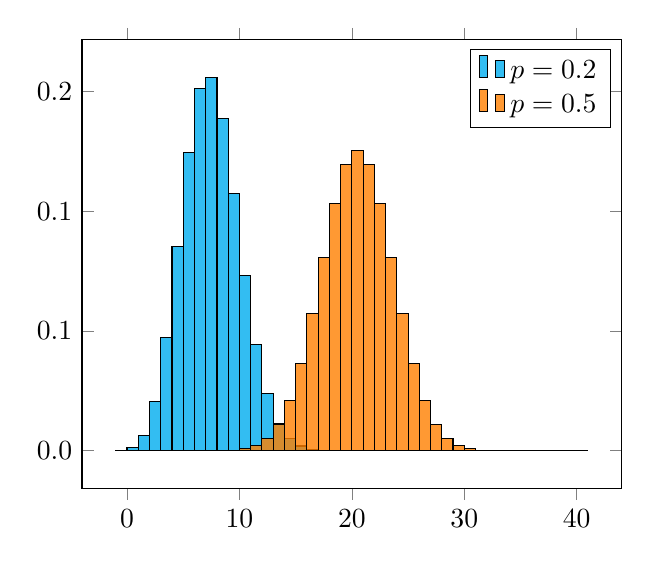
\begin{tikzpicture}[
		declare function={binom(\k,\n,\p)=\n!/(\k!*(\n-\k)!)*\p^\k*(1-\p)^(\n-\k);}
		]
		\begin{axis}[
			samples at={0,...,40},
			yticklabel style={
				/pgf/number format/fixed,
				/pgf/number format/fixed zerofill,
				/pgf/number format/precision=1
			},
			ybar=0pt, bar width=1
			]
			\addplot [fill=cyan, fill opacity=0.8] {binom(x,40,0.2)}; \addlegendentry{$p=0.2$}
			\addplot [fill=orange, fill opacity=0.8] {binom(x,40,0.5)}; \addlegendentry{$p=0.5$}
		\end{axis}
	\end{tikzpicture}
	\caption{Représentation graphiques de lois binomiales pour $n=40$ et différentes valeurs de $p$.}
\end{figure}

\begin{proposition}{}{}
	Si $X$ suit une loi binomiale $\mathscr{B}(n,p)$ alors :
	\begin{itemize}
		\item $\EX = np$
		\item $\sigma^2(X)=np(1-p)$
	\end{itemize}
\end{proposition}

\subsubsection{Loi géométrique}
\paragraph{Modèle :} On considère une succession  d'expériences indépendantes de Bernoulli, de type succès-échec que l'on notera respectivement S et E. La variable aléatoire $T$ est le temps d'attente du premier succès : l'événement $\underbrace{EE...E}_{k-1 \text{ échecs}}S  $ s'écrit donc $\{T=k\}$.

\begin{itemize}
	\item $T(\Omega) = \N^*$ 
	\item pour tout $k \in T(\Omega)$ :
	$$\prob(T=k)=(1-p)^{k-1}p$$
\end{itemize}

\begin{proposition}{}{}
	Si $T$ suit une loi géométrique $\mathscr{G}(p)$ où $p$ est la probabilité d'un succès, alors :
	\begin{itemize}
		\item $\mathbb{E}(T) = \frac{1}{p}$
		\item $\sigma^2(T)=\frac{1-p}{p^2}$
	\end{itemize}
\end{proposition}

\begin{theoreme}{}{}
	La loi géométrique est une loi sans mémoire : pour tout $(n,m) \in \N^2$, 
	$$\prob_{X>m}(X > m+n)=\prob(X>n)$$
\end{theoreme}

\subsubsection{Loi de Poisson}
\begin{definition}{}{}
	Une variable aléatoire $X$ suit une loi de \trouer{Poisson} de paramètre $\lambda >0$ (notée $\mathscr{P}(\lambda)$) si 
	\begin{itemize}
		\item $X(\Omega)=\N$ 
		\item pour tout $k \in \N$,  $$\prob(X=k)=e^{-\lambda}\frac{\lambda^k}{k!}$$
	\end{itemize}
\end{definition}

\paragraph{Modèle :} C'est la loi des \trouer{évènements rares} : elle est utilisée lorsqu'on considère le nombre de succès lors d'une répétition indépendante d'un grand nombre d'expériences ayant une probabilité faible de succès. Elle permet  d'approcher une loi binomiale lorsque $n$ est suffisamment grand et $p$ suffisamment petit (les conditions pratiques de l'approximation seront précisées plus tard dans ce document).

\begin{proposition}{}{}
	Si $X$ suit une loi de Poisson $\mathscr{P}(\lambda)$ alors :
	\begin{itemize}
		\item $\EX = \lambda$
		\item $\sigma^2(X)=\lambda$
	\end{itemize}
\end{proposition}

\subsection{Fonction génératrice}

\begin{definition}{}{}
	Soit $X \colon \Omega \to \N $ une variable aléatoire discrète à valeurs dans $\N$ .  La \trouer{fonction génératrice} de X est la série entière définie sur $[-1;1]$ par :
	$$g_X(t)=\mathbb{E}[t^X] =\sum _{n=0} ^{+\infty} \prob(X=n)t^n$$
	
\end{definition}

\begin{proposition}{}{}
	La fonction génératrice $g_X$ caractérise la loi de $X$ : pour tout $k \in \N $, 
	$$\prob(X=k)=\frac{1}{k!}g_X^{(k)}(0)$$
\end{proposition}

\begin{proposition}{}{}
	Si $X$ a pour fonction génératrice $g_X$  alors 
	$$\EX = g_X'(1)$$
\end{proposition}

On retrouve de la même façon les moments de $X$, s'ils existent, à partir de la fonction génératrice.

\begin{exemple}{}{}
	La fonction génératrice de quelques lois discrètes usuelles :
	\begin{enumerate}
		\item Loi uniforme sur $\{1;...;n\}$ : $g_X(t)=  \frac{t(1-t^n)}{n(1-t)}$
		\item Loi binomiale : $g_X(t)=  (tp + (1-p))^n$
		\item Loi géométrique : $g_X(t)=  \frac{tp}{1-t(1-p)}$
		\item Loi de poisson : $g_X(t) = e^{\lambda(t-1)}$
	\end{enumerate}
\end{exemple}


\subsection{Fonction caractéristique}

\begin{definition}{Fonction caractéristique}{}
La \trouer{fonction caractéristique} d'une variable aléatoire réelle $X$ est la fonction à valeurs complexes définie sur $\R$ par

$$\phi_{X}(t) =\mathbb{E}\left[e^{i tX}\right]=g_X(e^{i t})$$
\end{definition}


De même que pour la fonction génératrice, la fonction caractéristique caractérise la loi de $X$ et permet de calculer l'espérance : 
$$\EX = i\phi_X'(0)$$

\section{Avec plusieurs variables aléatoires}
\subsection{Vecteur de variables aléatoires}

Un vecteur de variables aléatoires est la données de $n$ variables aléatoires $(X_1,...,X_n)$. Pour $n=2$, on parlera de couple de variables aléatoires.

\begin{definition}{}{}
	Soit $(X,Y)$ un couple de variables aléatoires discrètes définies sur un espace $(\Omega,\prob)$. On appelle \trouer{loi conjointe} ou \trouer{loi mutuelle} de $(X,Y)$ la famille de valeurs 
	$$\prob(X=x,Y=y) = \prob(\{X=x\}\cap \{Y=y\}), \quad (x,y)\in X(\Omega) \times Y(\Omega)$$
\end{definition}

On pourra déterminer les lois marginales :

\begin{definition}{}{}
	Les \trouer{lois marginales} du couple $(X,Y)$ sont les lois des variables aléatoires $X$ et $Y$. Elles sont données par 
	$$\prob(X=x)=\sum_{y \in Y(\Omega)} \prob(\{X=x\}\cap \{Y=y\})$$
		$$\prob(Y=y)=\sum_{x \in X(\Omega)} \prob(\{X=x\}\cap \{Y=y\})$$
\end{definition}

\subsection{Variables aléatoires indépendantes}

\begin{definition}{}{}
	Soit $(X,Y)$ un couple de variables aléatoires définies sur un espace $\Omega$. Alors $X$ et $Y$ sont \trouer{indépendantes} si pour tout événement $A \in X(\Omega)$, $B \in Y(\Omega)$ alors
	$$\prob(X \in A, Y \in B)=\prob(X \in A) \times \prob(Y \in B)$$
	
\end{definition}

	On note aussi $\prob(X \in A, Y \in B) = \prob(\{X \in A\} \cap \{Y \in B\})$

\begin{proposition}{}{}
	Soit  $(X,Y)$ un couple de variables aléatoires indépendantes, $g$ et $h$ deux fonctions définies telles que $g(X)$ et $h(Y)$ existent. Alors $g(X)$ et $h(Y)$ sont deux variables aléatoires indépendantes.
\end{proposition}


\begin{proposition}{}{espindep}
		Soit  $(X,Y)$ un couple de variables aléatoires réelles discrètes. On suppose que $X$ et $Y$ admettent une espérance. Si $X$ et $Y$ sont \trouer{indépendantes}, alors $$\mathbb{E}(XY)=\mathbb{E}(X)\mathbb{E}(Y)$$
		La réciproque est fausse en général.
\end{proposition}

		\begin{exemple}{}{}
	Soit $X$ une variable aléatoire discrète telle que $\prob(X=0) = \prob(X=1) = \prob(X=-1) = \frac{1}{3}$. Soit $Y=\left\{\begin{array}{cl}
	0&\text{si $X \neq 0$}\\
	1 &\text{si $X=0$}
	\end{array}\right.$ Alors $\mathbb{E}(XY) = 0$, $\mathbb{E}(X) = 0$ donc $\mathbb{E}(XY)=\mathbb{E}(X)\mathbb{E}(Y)$ alors que par définition, $X$ et $Y$ ne sont pas indépendantes.
\end{exemple}

\subsection{Covariance}

On définit ainsi un indicateur mesurant l'écart par rapport à l'indépendance :

\begin{definition}{Covariance}{}
	Soit un couple de variable aléatoires $(X,Y)$ : la \trouer{covariance} de $X$ et $Y$ est le réel 
	$$\cov(X,Y) = \mathbb{E} \left[ (X-\EX)(Y-\mathbb{E}(Y)) \right] = \mathbb{E}(XY)-\mathbb{E}(X)\mathbb{E}(Y)$$
\end{definition}

La propriété \ref{pr:espindep} se reformule ainsi : 

\begin{proposition}{}{}
	Si $X$ et $Y$ sont indépendantes, alors $\cov(X,Y)=0$.
\end{proposition}

La variance n'est pas linéaire, mais la variance d'une somme fait intervenir la covariance :

\begin{proposition}{}{}
	Soit un couple de variable aléatoires $(X,Y)$ et $a,b$ deux réels :
	$$\var(aX+bY)=a^2\var(X)+b^2\var(Y)+2ab \times \cov(X,Y)$$
\end{proposition}

Il est utile de retenir le corollaire suivant : si $X$ et $Y$ sont \trouer{indépendantes}, alors $$\var(X+Y)=\var(X)+\var(Y)$$

\begin{proposition}{Inégalité de Cauchy-Schwarz}{}
	Soit un couple de variable aléatoires $(X,Y)$ admettant chacune un moment d'ordre 2. Alors 
$$\cov(X,Y)^2 \leq \var(X)\var(Y)$$	

\end{proposition}

\begin{definition}{Coefficient de corrélation linéaire}{}
	Soit un couple de variable aléatoires $(X,Y)$ admettant chacune un moment d'ordre 2 et des variances non nulles. Alors le coefficient de corrélation linéaire est 
	
	$$\rho(X,Y)=\frac{\cov(X,Y)}{\sqrt{\var(X)\var(Y)}}$$
\end{definition}

D'après l'inégalité précédente, ce coefficient est dans $[-1;1]$. Il mesure le degré de dépendance linéaire entre les deux variables : proche de $-1$ ou $1$, ce degré est élevé ; si $\rho(X,Y)=0$, on dit que $X$ et $Y$ sont non linéairement corrélées.


					
%					On observera une représentation graphique de six cas typiques en figure \ref{fig:exemplescorrelation}.
%					
%					\begin{figure}[h!]
%						\centering
%						\includegraphics[width=0.5\linewidth]{exemples}
%						\caption[]{Différents cas de figures}
%						\label{fig:exemplescorrelation}
%					\end{figure}


		
\subsection{Somme de variables aléatoires indépendantes}

\begin{proposition}{}{}
	Soit  $(X,Y)$ un couple de variables aléatoires réelles discrètes. Si $X$ et $Y$ sont indépendantes, alors $$ \prob(X+Y=s) = \sum_i \prob(X=x_i) \prob(Y=s-x_i)$$
\end{proposition}

\begin{proposition}{Fonctions caractéristiques et génératrices d'une somme}{}
	Soit  $(X,Y)$ un couple de variables aléatoires réelles. Si $X$ et $Y$ sont indépendantes, alors 
	\begin{enumerate}
		\item Pour tout $t \in [-1;1]$, $g_{X+Y}(t)=g_X(t)g_Y(t)$
		\item Pour tout $t \in \R $, $\phi_{X+Y}(t)=\phi_X(t)\phi_Y(t)$
	\end{enumerate}

\end{proposition}

\subsection{Quelques exemples}

	\begin{exemple}{}{}
		Soit $X$ et $Y$ deux variables aléatoires indépendantes suivant une loi uniforme sur $\{1;...;n\}$. Alors la variable $Z=X+Y$ suit une loi  triangulaire : 
		\begin{itemize}
			\item si $z \leq n+1$,  $\prob(Z=z)= \frac{z-1}{n^2}$
			\item si $z > n+1$,  $\prob(Z=z) = \frac{2n-z+1}{n^2}$
		\end{itemize}
	\end{exemple}

%\begin{proposition}
%Soient $(X_1,...,X_n)$ 	des variables aléatoires indépendantes suivant chacune une même loi de Bernoulli de paramètre $p$. Alors la variable $S=\sum_{i=1}^{n} X_i$ suit une loi binomiale de paramètres $(n,p)$.
%\end{proposition}

\begin{proposition}{}{}
	Soit  $(X,Y)$ un couple de variables aléatoires \trouer{indépendantes} telles que $X$ suit une loi de Poisson $\mathcal{P}(\lambda_1)$, $Y$ suit une loi de Poisson $\mathcal{P}(\lambda_2)$. Alors $X+Y$ suit une loi de Poisson $\mathcal{P}(\lambda_1+\lambda_2)$
\end{proposition}


